\documentclass{book}
\usepackage{geometry}
\usepackage[utf8]{inputenc} % UTF-8 unterstützung
\geometry{papersize={170mm,240mm},total={140mm,200mm},top=21mm,bindingoffset=10mm}
\usepackage{etex}
\usepackage{ngerman}
\usepackage{times}
\usepackage{amsmath}
\usepackage{amssymb}
\usepackage{amsfonts}
\usepackage{amsthm}
\usepackage{graphicx}
\usepackage{fancyhdr}
\usepackage{textcomp}
\usepackage[all]{xy}
\usepackage{txfonts}
\usepackage{alltt}
\usepackage{verbatim}
\usepackage{paralist}
\usepackage{makeidx}
\usepackage{array}
\usepackage{hyperref}
\usepackage{tikz}
\usepackage{xcolor}
\usepackage{multicol}
\usepackage{listings}
\lstdefinestyle{Matlab}{
  numbers=left,
  belowcaptionskip=1\baselineskip,
  breaklines=true,
  frame=L,
  xleftmargin=\parindent,
  language=Matlab,
  showstringspaces=false,
  basicstyle=\footnotesize\ttfamily,
  keywordstyle=\bfseries\color{green!40!black},
  commentstyle=\itshape\color{purple!40!black},
  identifierstyle=\color{blue},
  stringstyle=\color{orange},
  numberstyle=\ttfamily\tiny
}
\lstdefinestyle{C}{
  belowcaptionskip=1\baselineskip,
  breaklines=true,
  frame=L,
  xleftmargin=\parindent,
  language=C,
  showstringspaces=false,
  basicstyle=\footnotesize\ttfamily,
  keywordstyle=\bfseries\color{green!40!black},
  commentstyle=\itshape\color{purple!40!black},
  identifierstyle=\color{blue},
  stringstyle=\color{orange},
  numberstyle=\ttfamily\tiny
}

\usepackage{caption}
\usepackage{subcaption}
\usepackage{epstopdf}
\usepackage{standalone}
\usepackage[backend=bibtex]{biblatex}
\addbibresource{MonteCarlo.bib}



\begin{document}
\title{Monte Carlo Methode}
\author{Dorian Amiet, Hannes Badertscher}
\date{}
\maketitle



\chapter{Die Monte Carlo Methode}
\rhead{Die Monte Carlo Methode}
\begin{refsection}

\section{Einleitung}
Der Monte Carlo Algorithmus ist ein Verfahren zur Lösung numerischer Probleme durch das Ziehen von Zufallszahlen. Die Idee, mathematische bzw. physikalische Probleme mit einem stochastischen Sampling-Verfahren zu approximieren stammt vom polnisch-amerikanischen Mathematiker Stanisław Marcin Ulam (1909 -- 1984), welcher zu dieser Zeit im Los Alamos National Labaratory arbeitete. Seine Idee, und wie es dazu kam, beschrieb er folgendermassen: \\

\begin{quote}
\textit{“The first thoughts and attempts I made to practice [the Monte Carlo method] were suggested by a question which occurred to me in 1946 as I was convalescing from an illness and playing solitaires. The question was what are the chances that a Canfield solitaire laid out with 52 cards will come out successfully? After spending a lot of time trying to estimate them by pure combinatorial calculations, I wondered whether a more practical method than “abstract thinking” might not be to lay it out say one hundred times and simply observe and count the number of successful plays. This was already possible to envisage with the beginning of the new era of fast computers, and I immediately thought of problems of neutron diffusion and other questions of mathematical physics, and more generally how to change processes described by certain differential equations into an equivalent form interpretable as a succession of random operations. Later... [in 1946, I ] described the idea to John von Neumann and we began to plan actual calculations.”} - Stan Ulam, 1983
\end{quote}

Monte Carlo Methoden kommen überall zum Einsatz, wenn deterministische Algorithmen entweder zu komplex sind oder gar nicht existieren. Dank zunehmender Rechenleistung sind in den letzten Jahren Simulationen wie globale Klimamodelle möglich geworden. Typische Anwendungen des Monte Carlo Algorithmus umfassen u.a.

\begin{itemize}
	\item Numerische Integration
	\item Simulation von dynamischen Prozessen
	\item Simulation von Gleichgewichtszuständen (z.B. mit Metropolis-Algorithmus)
	\item Statistische Untersuchung von Zufallsverteilungen
\end{itemize}

\section{Funktionsprinzip}
Die Monte Carlo Methode ist ein Überbegriff für verschiedene Algorithmen zur numerischen Berechnung / Simulation mittels Zufallsereignissen. Ein weit verbreiteter und sehr flexibler Ansatz ist das sogenannte Hit-or-Miss Verfahren. Dabei werden Zufallszahlen generiert und geprüft, ob diese eine bestimmte Bedingung erfüllen oder nicht. Mit dem Verhältnis Hit / Miss wird das gewünschte Ergebnis approximiert. 

\subsection{Numerische Integration} \label{subsec:numIntegration}
Einer der wichtigsten Anwendungsbereiche der Monte Carlo Methode ist die numerische Berechnung von Integralen. Dazu werden innerhalb des Definitionsbereich der zu integrierenden Funktion Zufallsereignisse generiert. Generell kann ausgesagt werden, dass das Integral

\begin{equation}
	I = \int_a^b f(x) dx
\end{equation} 

mit $N$ im Intervall $[a,b]$ gleichverteilten Zufallszahlen $x_i$ durch

\begin{equation}
	\hat{I} = (b-a) \cdot \frac{1}{N} \sum_{i=1}^{N} f(x_i)
\end{equation}

approximiert werden kann. Der relative Fehler sinkt dabei mit $\frac{1}{\sqrt{N}}$. Während für analytisch lösbare Integrale und solche mit kleinen Dimensionen ($\leq 4$) andere Möglichkeiten oft schneller sind, ist die Monte Carlo Methode besonders bei hohen Dimensionen oder sehr komplizierten Integrationsgrenzen verbreitet. \\

Der Algorithmus lässt sich sehr einfach beschreiben:

\begin{enumerate}
	\item Finde das Maximum $f_{max}$ der Funktion $f(x)$.
	\item Erzeuge $N$ im Intervall $[a,b]$ gleichverteilte Zufallszahlen $x_i$.
	\item Erzeuge für jedes $x_i$ ein in $[0,f_{max}]$ gleichverteiltes $y_i$.
	\item Falls $y_i < f(x_i)$ wird das $x_i$ akzeptiert, sonst verworfen.
	\item Wenn $N^*$ die Anzahl der akzeptierten $x_i$ ist, dann ist $F = \frac{N^*}{N}(b-a)f_max$.
\end{enumerate}

Abbildung \ref{fig:integration_histogram} zeigt eine beliebige Funktion (rot), sowie die akzeptierten Ereignisse (blau) und die nicht akzeptierten Ereignisse (grün). \\

\begin{figure}[htbp]
	\centering
	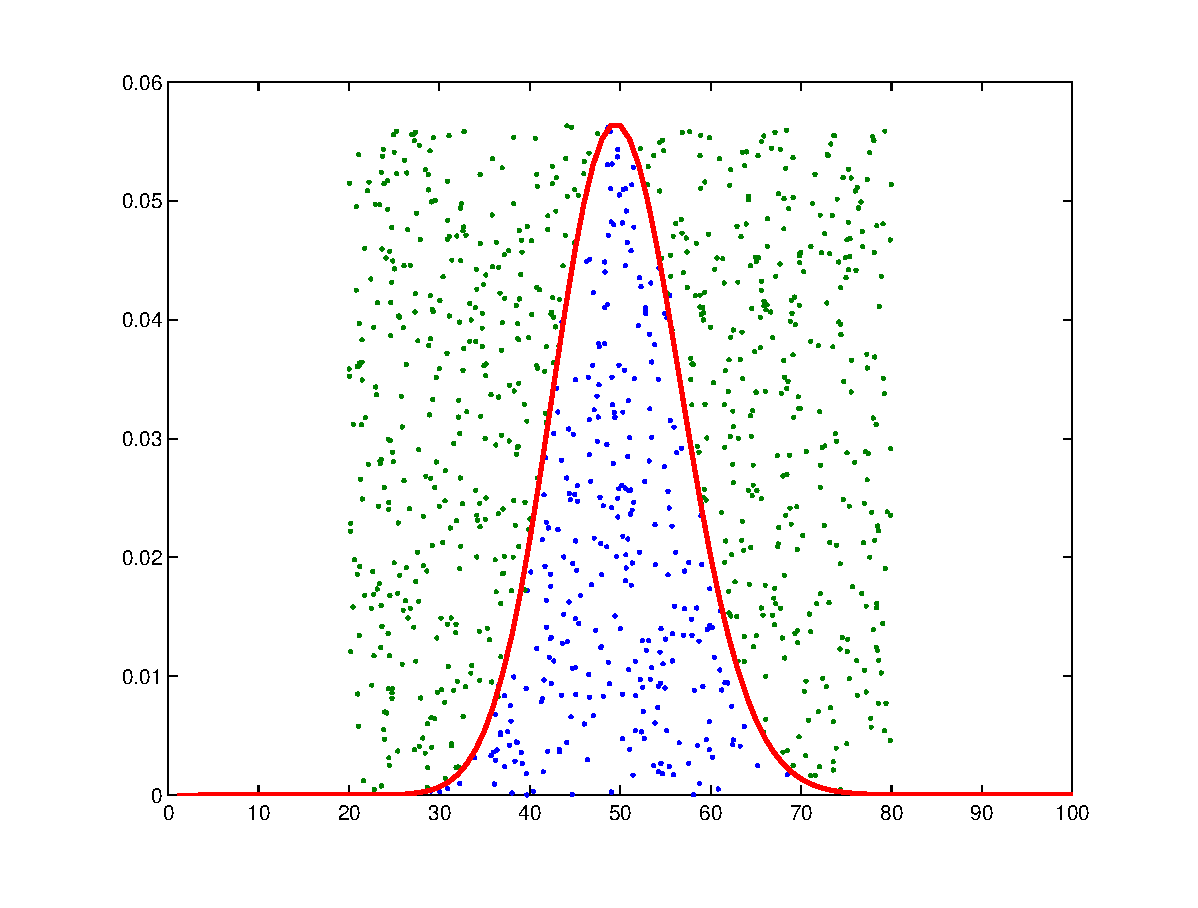
\includegraphics[width=7cm]{images/integration_poisson.eps}
	\caption{Monte Carlo Integration einer Funktion}
	\label{fig:integration_histogram}
\end{figure}

Besonders in der Teilchenphysik - aus welcher die Monte Carlo Methode bekannterweise stammt - wird die Monte Carlo Methode sehr häufig angewandt. Meist ist man dabei nicht nur am numerischen Resultat, sondern auch an den einzelnen Ereignissen, welche zu diesem Resultat geführt haben, interessiert. Dazu wird der Algorithmus leicht modifiziert. Die Zufallszahlen $x_i$ werden neu nicht gleichverteilt, sondern mit der Wahrscheinlichkeitsdichtfunktion $f(x)$ bzw. der Verteilungsfunktion $F(x)$ erzeugt. Das Histogramm dieser $x_i$ entspricht der mit $N/F$ normierten Funktion $f(x)$. Das Resultat $F$ kann also durch einen Vergleich des Histogramms mit der Funktion $f(x)$ bestimmt werden. Der Vorteil dieser Methode ist, dass so die Ereignisse $x_i$ mit der richtigen Verteilung bekannt sind und ausgewertet werden könne.

\subsection{Abschätzung des Wertes von Pi}
Als Einführungsbeispiel für die Monte Carlo Methode wird die Zahl $\pi$ mit einer Hit-or-Miss Methode abgeschätzt. Ein Kreis mit Radius $r$ hat eine Grundfläche von $A_{\text{Kreis}} = \pi r^{2}$.  Damit muss in einem Intervall von $[-r,+r]$ integriert werden, was eine Fläche von $A_{\text{Quadrat}} = 4r^2$ ergibt. Damit lässt sich $\pi$ approximieren als

\begin{equation}
	\hat{\pi} = \frac{A_{\text{Kreis}}}{r^2} = 4 \frac{A_{\text{Kreis}}}{A_{\text{Quadrat}}}
\end{equation}

Das Verhältnis der Fläche des Kreises zur Fläche des Quadrats entspricht der Wahrscheinlichkeit, dass ein Paar Zufallszahlen $(x_i,y_i)$ mit $x_i,y_i \leq r$ innerhalb des Kreises mit Radius $r$ liegen. Dies wird mit folgender Formel überprüft:

\begin{equation}
	x^2 + y^2 \leq r
	\label{equ:innerhalbKreis}
\end{equation}

\begin{figure}[htbp]
	\centering
	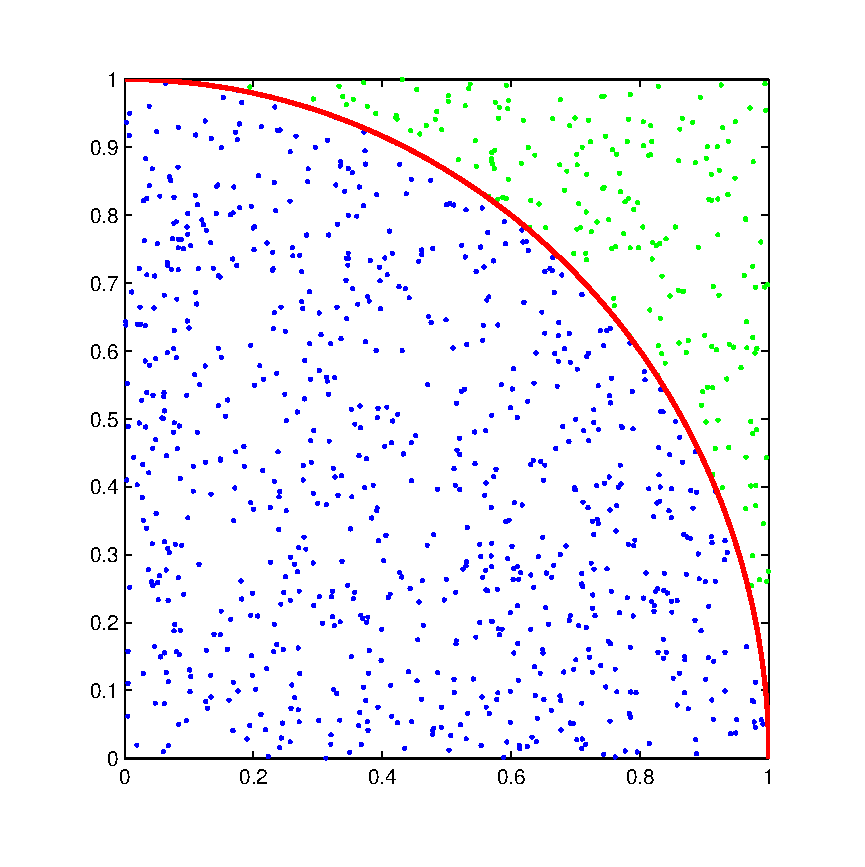
\includegraphics[width=6cm]{images/kreis_hitmiss.eps}
	\caption{Kreis}
	\label{fig:KreisHitMiss}
\end{figure}

Dank der Symmetrie des Kreises kann das Problem offensichtlich auf den ersten Quadranten reduziert werden. Für $N$ Iterationen, von welchen $k$ die Bedingung \ref{equ:innerhalbKreis} ergibt sich somit folgende Abschätzung für Pi:

\begin{equation}
	\hat{\pi} = 4 \cdot \frac{k}{N}
\end{equation}



\section{Implementation}
\subsection{Implementation in C}
Die Implementation dieses Beispiels in C ist relativ kurz und übersichtlich: Über $N$ Iterationen wird jeweils ein Paar Zufallszahlen $(x,y)$ generiert und die Gleichung \ref{equ:innerhalbKreis} $x^2 + y^2$ berechnet. Ist das Resultat $<1$ wird eine Summe erhöht. Das Resultat ist schlussendlich die Summe geteilt durch die Anzahl Iterationen $N$ mal 4 Da diese Lösung nicht parallel abläuft, steigt der Rechenaufwand linear mit der Anzahl Iterationen. \\


\clearpage
\begin{figure}[h]
    \centering
    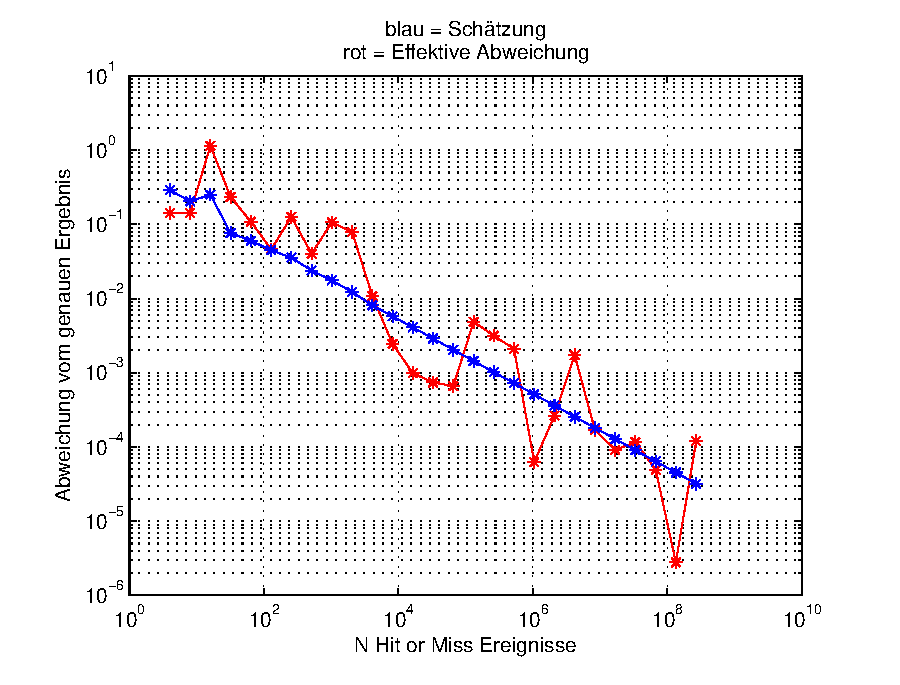
\includegraphics[width=8cm]{images/Fehler.eps}
    \caption{Betrag der Abweichung}
    \label{fig:Fehler}
\end{figure}

Die Genauigkeit wird, wie zu erwarten ist, mit einem Faktor $1/\sqrt{N}$ zunehmen. Der relative Fehler kann mittels Effizienz $\epsilon$ und Anzahl angenommene Ereignisse $k$ abgeschätzt werden.

\begin{equation}
	\epsilon = \frac{k}{N}
\end{equation} 

\begin{equation}
	\text{Relativer Fehler} = \sqrt{\frac{1-\epsilon}{k}}
	\label{eq:relativer_Fehler}
\end{equation}

Anhand der beiden Formeln können einige wichtige Erkenntnisse gewonnen werden. So ist es von Vorteil, die Effizienz so nahe an eins wie möglich zu halten. Dies wird erreicht, indem das Zielgebiet $\Omega$ möglichst klein gehalten wird. Für die Plausibilitätsüberprüfung werden die Extremfälle betrachtet. Das kleinstmögliche $\Omega$ ist gerade die Zielfunktion selber. Dabei wird jedes mögliche HM-Ereignis ein Hit. Dies führt dazu, dass $k = N$ und somit $\epsilon$ = 1. Der relative Fehler ist somit bereits nach einer Iteration bei null. Bei einem sehr grossen $\Omega$ wird die Wahrscheinlichkeit, dass ein Hit generiert wird, sehr klein. Somit bleibt $k$ auch nach vielen Operationen klein, wobei $N$ gross wird. $\epsilon$ wird dabei fast null und der relative Fehler belauft sich auf rund $1/\sqrt{k}$.\\

\subsection{Genauigkeit des Schätzers}

Um die Genauigkeit der Fehlerabweichung besser abschätzen zu können, wird die Simulation 1000 mal durchgeführt und die gemittelte effektive Abweichung mit der Schätzung verglichen.\\

\clearpage
\begin{figure}[h]
    \centering
    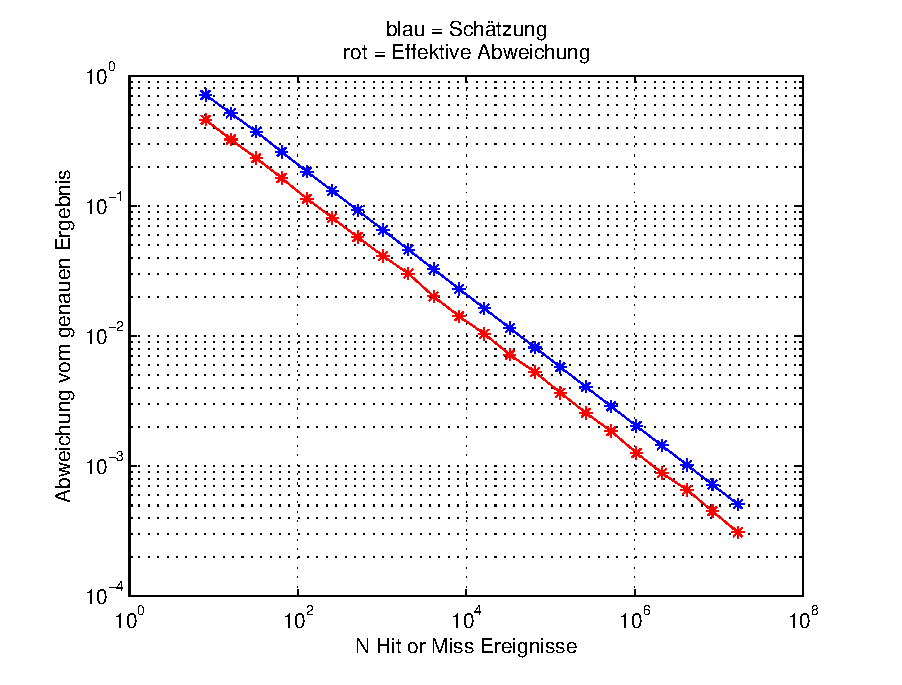
\includegraphics[width=8cm]{images/Fehler_gemittelt.eps}
    \caption{Betrag der Abweichung, gemittelt}
    \label{fig:Fehler_gemittelt}
\end{figure}

Dabei zeigt sich, dass die Schätzung ca. um den Faktor 2 höher liegt als die Abweichungen der Simulationsergebnisse. Zumindest die Grössenordnung des Schätzers stimmt somit. Um zu illustrieren, wie der Faktor zustande kommen könnte, wird ein Histogramm der Fehlerabweichung gemacht. Dazu werden eine Million Simulationen mit N=1000 durchgeführt und in die Beträge der Abweichung in ein Histogramm eingetragen. In Abbildung \ref{fig:Histogramm} ist ersichtlich, dass die Streuung ziemlich hoch ist. Es tauchen Werte auf, welche das zehnfache des Schätzers betragen. Somit ist der Schätzer sowieso nur als Grössenordnung zu verstehen, da ein Einzelnes Simulationsergebnis wesentlich ungenauer sein kann.

Der Mittelwert der Abweichungen liegt bei 0.0414, der Schätzer prognostiziert 0.0661. Dies entspricht einem Faktor von rund 0.63. Die Formel \ref{eq:relativer_Fehler}, welche den relativen Fehler Schätzt, könnte in diesem Beispiel mit der Konstante 0.6 ergänzt werden, womit die Schätzung sehr genau stimmen würde. Ob dieser Faktor nur in diesem Beispiel oder generell gilt, wird nicht weiter untersucht.

\begin{figure}[h]
    \centering
    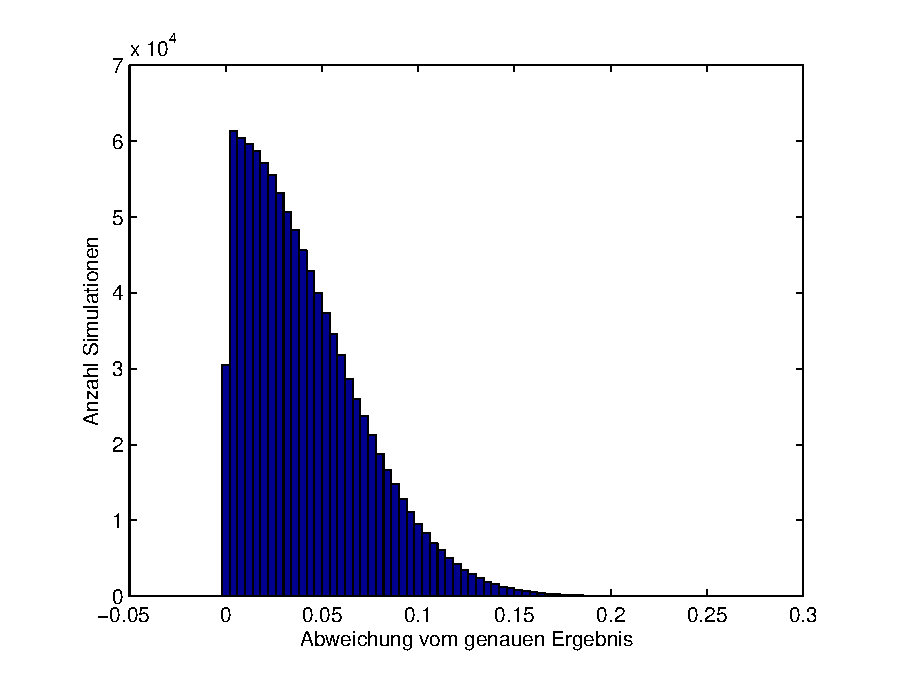
\includegraphics[width=8cm]{images/Histogramm.eps}
    \caption{Beträge des Effektiven Fehlers bei N = 1000, Fehlerschätzung = 0.0165}
    \label{fig:Histogramm}
\end{figure}



\subsection{Implementation in OpenCL}
Bei der Monte Carlo Analyse werden sehr viele komplett unabhängige Berechnungen durchgeführt. Dadurch ist OpenCL perfekt geeignet, um das Problem zu parallelisieren. Die grösste Schwierigkeit dabei ist die Generierung von Zufallszahlen auf der GPU. 

\subsubsection{Ansatz I: Zufallszahlen auf CPU}
Die einfachste Lösung für das Problem ist es, auf der CPU qualitativ hochwertige Zufallszahlen zu generieren und in einem Array an OpenCL zu übergeben. Jeder Worker liest seine zwei Zufallszahlen aus und rechnet das Resultat für diesen Punkt aus. So ist sichergestellt, dass die Zufallszahlen wirklich zufällig sind und das Resultat gegen den korrekten Wert konvergiert. Die Nachteile sind, dass die Berechnung der Zufallszahlen seriell und somit langsam ist, sowie der hohe Speicherverbrauch. Dieser kann um einen Faktor 2 reduziert werden, indem nur eine Zufallszahl übergeben wird und jeder Worker sich eine zweite Zahl berechnet. \\

Wird diese Variante mit C bzw. OpenCL umgesetzt, stellen sich die erwarteten Resultate ein: Die Rechenzeit steigt linear mit der Anzahl Punkte, die Berechnung ist jedoch deutlich schneller als bei serieller Berechnung auf der CPU. Mit 48.909 Mio Berechnungen pro Sekunde ist die parallelisierte Version um Faktor 5 schneller  als die serielle Implementation.

\begin{figure}[htbp]
	\centering
	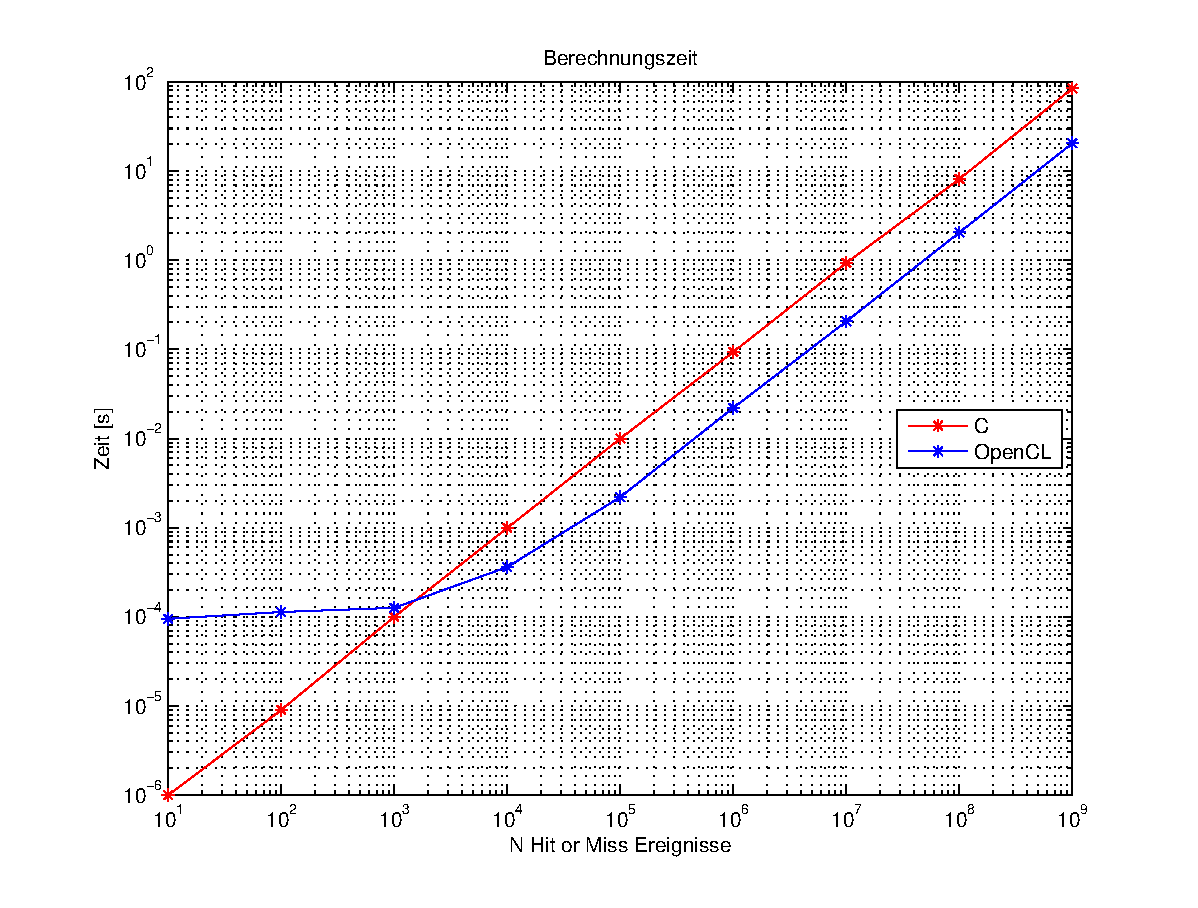
\includegraphics[width=8cm]{images/Berechnungszeit_OpenCL.eps}
	\caption{Berechnungszeit mit OpenCL}
	\label{fig:OpenCL_Berechnungszeit}
\end{figure}


\subsubsection{Ansatz II: Zufallszahlen auf GPU}
Da Zufallszahlen mathematisch berechnet werden, liegt es nahe, diese auf der GPU zu berechnen. Als Startwert (seed), kann z.B. die Worker-ID verwendet werden. So verfügen alle Worker über unabhängige Zufallszahlen. Die meisten Algorithmen sind jedoch nur dazu geeignet, von einem Startwert aus eine lange Folge unabhängiger Zufallszahlen zu berechnen. Wird der Algorithmus nach nur 2 Werten mit einem anderen Startwert neu gestartet, ergibt sich kein besonders zufälliges Muster. Abbildung \ref{fig:OpenCL_ID_Seed} zeigt den Ausgang eines Zufallszahlengenerators in Abhängigkeit des Startwertes. Werden diese Werte für die Monte Carlo Simulation verwendet, wird das Ergebnis nicht gegen den korrekten Wert konvergieren. 

\begin{figure}[htbp]
	\centering
	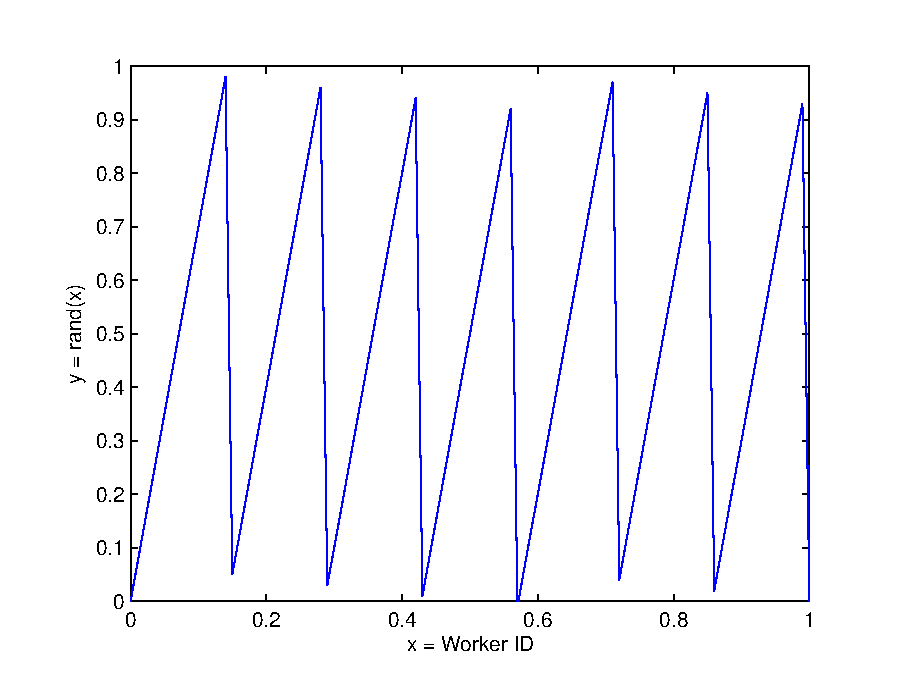
\includegraphics[width=8cm]{images/idAsSeed.eps}
	\caption{Zufallszahlen auf GPU mit Worker-ID als Seed}
	\label{fig:OpenCL_ID_Seed}
\end{figure}

\subsubsection{Ansatz III: Mischform}
Die beste Lösung liegt in einer Mischform der beiden Ansätze: Auf der CPU wird eine geringe Anzahl qualitativ hochwertiger Zufallszahlen generiert. Mit diesen können Zufallszahlen-Generatoren auf der GPU initialisiert werden. Damit sich dieser Aufwand lohnt, wird pro Worker nicht nur ein Punkt berechnet, sondern eine Serie von Punkten. Das empfohlene Vorgehen lautet wie folgt:
\begin{enumerate}
	\item Abschätzen der Anzahl nötiger Iterationen $N$.
	\item Bestimmen des Zielsystems und der Anzahl parallel ausführbarer Workers $M$.
	\item Generieren von $M$ hochwertiger Zufallszahlen auf der CPU.
	\item Übergabe dieser $M$ Zahlen an OpenCL, Start des Kernels.
	\item Jeder Worker berechnet $N/M$ Punkte und gibt das Resultat zurück.
	\item Zusammenführen und Auswerten der Resultate der einzelnen Worker auf der CPU.
\end{enumerate}

Mit diesem Verfahren lässt sich die vorhandene Hardware gut ausnutzen, ohne Genauigkeit durch schlechte Zufallszahlen zu verlieren. 

\clearpage
\section{Zufallszahlengeneratoren} 

\begin{quote}
\textit{“Anyone who considers arithmetical methods of producing random digits is, of course, in a state of sin.”} - John von Neumann, 1951
\end{quote}

Die Generierung von Zufallszahlen ist absolut essentiell für die Monte Carlo Methode. In der analogen Welt bestehen verschiedene hervorragende Zufallsgeneratoren, u.a. das thermische Widerstandsrauschen oder radioaktive Zerfallsvorgänge. So gab es in der Vergangenheit Ansätze, in welchen die Strahlung einer radioaktiven Quelle gemessen wurde und daraus eine Folge von Zufallszahlen generiert wurde. Heute werden eher Rauschgeneratoren mit Widerständen oder Dioden verwendet. In digitalen Schaltungen wird teilweise der Ausgang eines metastabilen Flip-Flop als Zufallszahlengenerator verwendet.\\

In Software ist es deutlich schwieriger, ``gute'' Random Number Generators (RNGs) zu realisieren. Technisch gesehen sind Software RNGs immer \textit{Pseudo} Random Number Generators (pRNGs),  denn der Ausgangswert eines deterministischen Programms kann per Definition nicht zufällig sein. Die Schwierigkeit ist es, Zahlen zu generieren, die aus der Perspektive des Anwenders komplett zufällig sind, obwohl sie eindeutig mathematisch definiert sind.

\subsection{Random-Device} \label{subsec:RandomDev}

Auf Unix-Systemen steht mit dem sog. Random-Device (/dev/random) ein Zufallszahlengenerator sehr hoher Güte zur Verfügung. Dieser sammelt das Rauschen von Gerätetreibern in einem Entropie-Pool und generiert daraus Zufallszahlen, welche auch höchsten Anforderungen im Bereich der Kryptografie genügen. Der Nachteil ist, dass sobald dieser Entropie-Pool erschöpft ist keine Zufallszahlen mehr generiert werden können. Mit dem Device /dev/urandom wurde Abhilfe geschaffen, was jedoch mit dem Nachteil erkauft wird, dass beim Unterschreiten einer gewissen Entropie-Schwelle nur Pseudozufallszahlen generiert werden, welche unter Umständen von einem potentiellen Angreifer berechnet werden könnten. Den meisten Anforderungen genügt dies jedoch trotzdem. \\

Das Random-Device kann von einem Programm wie ein File eingebunden werden und Zufallszahlen daraus gelesen werden. Für viele Anwendungen ist dies klar zu langsam, weshalb häufig das Random-Device nur als Seed für einen Pseudo-Random-Number-Generator verwendet wird.

Ein Code-Snippet zur Verwendung des Random-Device ist im Github-Repository \cite{rng:githubRepo} zu finden.


\subsection{Multiplikativ kongruentielle Generatoren (LCG)} \label{subsec:LCG}
Eine der populärsten Methoden zur Generierung von Zufallszahlen ist die multiplikativ kongruentielle Methode. Solche Generatoren werden häufig als \textit{linear congruential generator (LCG)} bezeichnet. Dabei werden Zufallszahlen rekursiv nach folgender Vorschrift berechnet:

\begin{equation}
	x_{i+1} = \left( a x_{i} + b \right) \mod{m}
	\label{equ:lcg_equation}
\end{equation}

Der Generator ist durch den Startwert $x_1$, den Faktor $a$, das Inkrement $b$ und das Modul $m$ vollständig bestimmt. Ein LCG generiert Zufallszahlen zwischen $0$ und $m-1$. Für viele Zwecke sind gleichverteilte Zufallszahlen zwischen $0$ und $1$ gefragt. Diese werden wie folgt berechnet:

\begin{align}
	y_i &= \frac{x_i}{m} \: &\text{for approx. uniformly distributed numbers  in } [0,1)\\
	y_i &= \frac{x_i}{m-1} \: &\text{for approx. uniformly distributed numbers in [0,1]}
\end{align} 


LCG Generatoren sind sehr stark von der Wahl der Konstanten $a$,$b$,$m$ abhängig. Eine suboptimale Wahl kann zu einer sehr geringen Periode und einer eindeutigen Korrelation aufeinanderfolgender Zahlen führen. Abbildung \ref{fig:lcg_verteilung} verdeutlicht dies anhand eines LCG mit $a=11$, $b=0$ und $m=64$. \\

\begin{figure}[h]
	\centering
	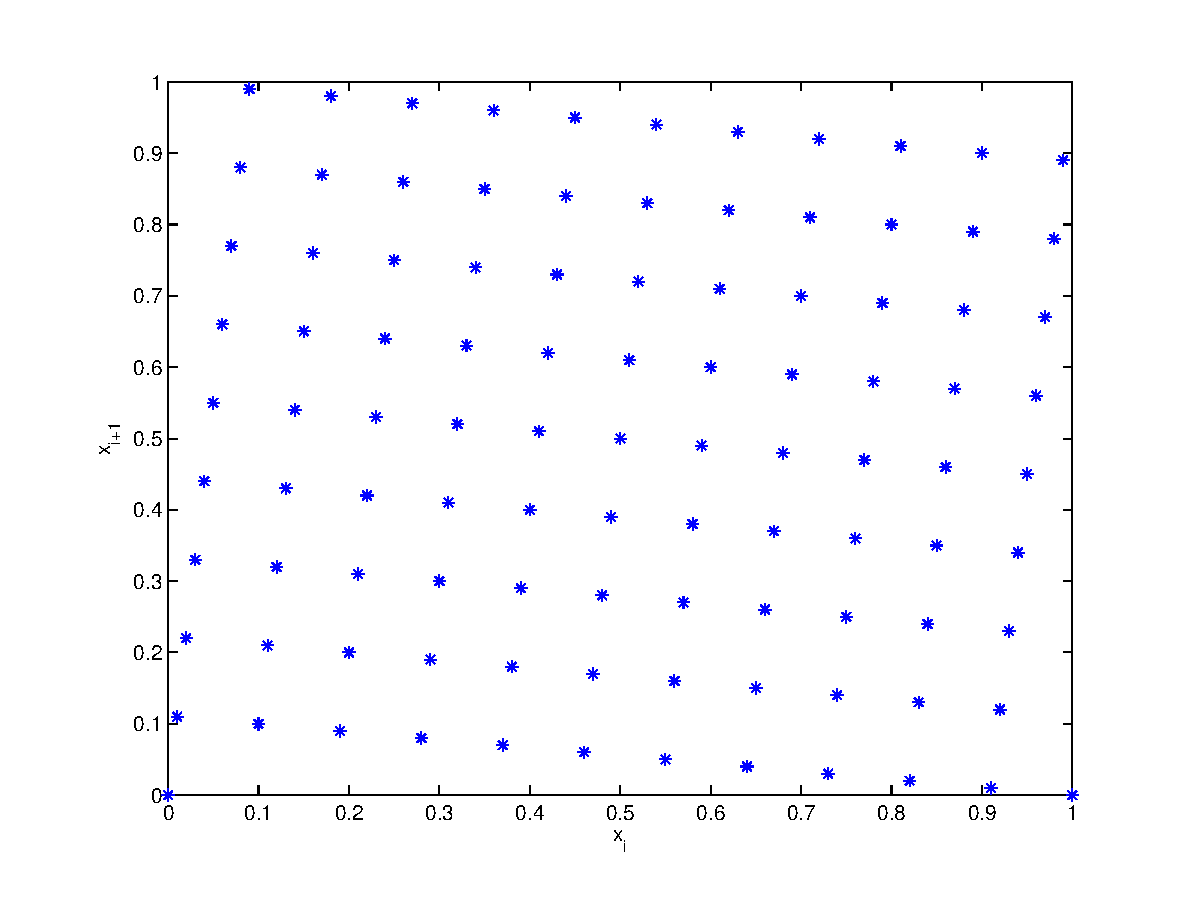
\includegraphics[width=8cm]{images/lcg.eps}
	\caption{Verteilung aufeinanderfolgender Zufallszahlen eines LCG mit $a=11$, $b=0$, $m=64$}
	\label{fig:lcg_verteilung}
\end{figure}

\subsubsection{Die IBM RANDU-Funktion}
Ein bekanntes Beispiel für schlecht entwickelte LCG Generatoren ist die Funktion \textit{RANDU}, welche ab den 60er-Jahren eine Standardfunktion auf dem IBM System/360 war. Diese nutzte einen LCG-Algorithmus gemäss folgender Gleichung:

\begin{equation}
	x_{i+1} = \left( 65539 \: x_i \right) \mod{2^{31}}
	\label{equ:ibm_randu}
\end{equation}

Mit $m = 2^{31}$ reduziert sich die Modulo-Operation in einem 32-bit System auf einen kontrollierten Overflow. Mit $a = 65539 = 2^{16} + 3 = 10\cdots011_{\text{bin}}$ wird die Multiplikation zu Additionen und Bit-Shifts vereinfacht. Der Algorithmus ist damit hocheffizient, hat aber folgendes Problem. \\

Aus der Zuordnungsvorschrift
\begin{equation*}
	x_{i+1} = (2^{16} + 3) x_i
\end{equation*}
folgt für zwei Iterationen:
\begin{align*}
	x_{i+2} &= (2^{16} + 3) x_{i+1} \\
	 &= (2^{16} + 3)^2 x_i \\
	 &= [6 (2^{16} + 3) - 9] x_i
\end{align*}

und somit gilt:
\begin{equation}
	x_{i+2} = 6 x_{i+1} - 9 x_i
\end{equation}

für alle $k$. Diese hohe Korrelation ist in Abbildung \ref{fig:IBMRandu} dargestellt. Donald E. Knuth bezeichnet den Generator deshalb als \textit{``really horrible''} \cite[p.173]{rng:KnuthVol2}. \\

\begin{figure}[htbp]
	\centering
	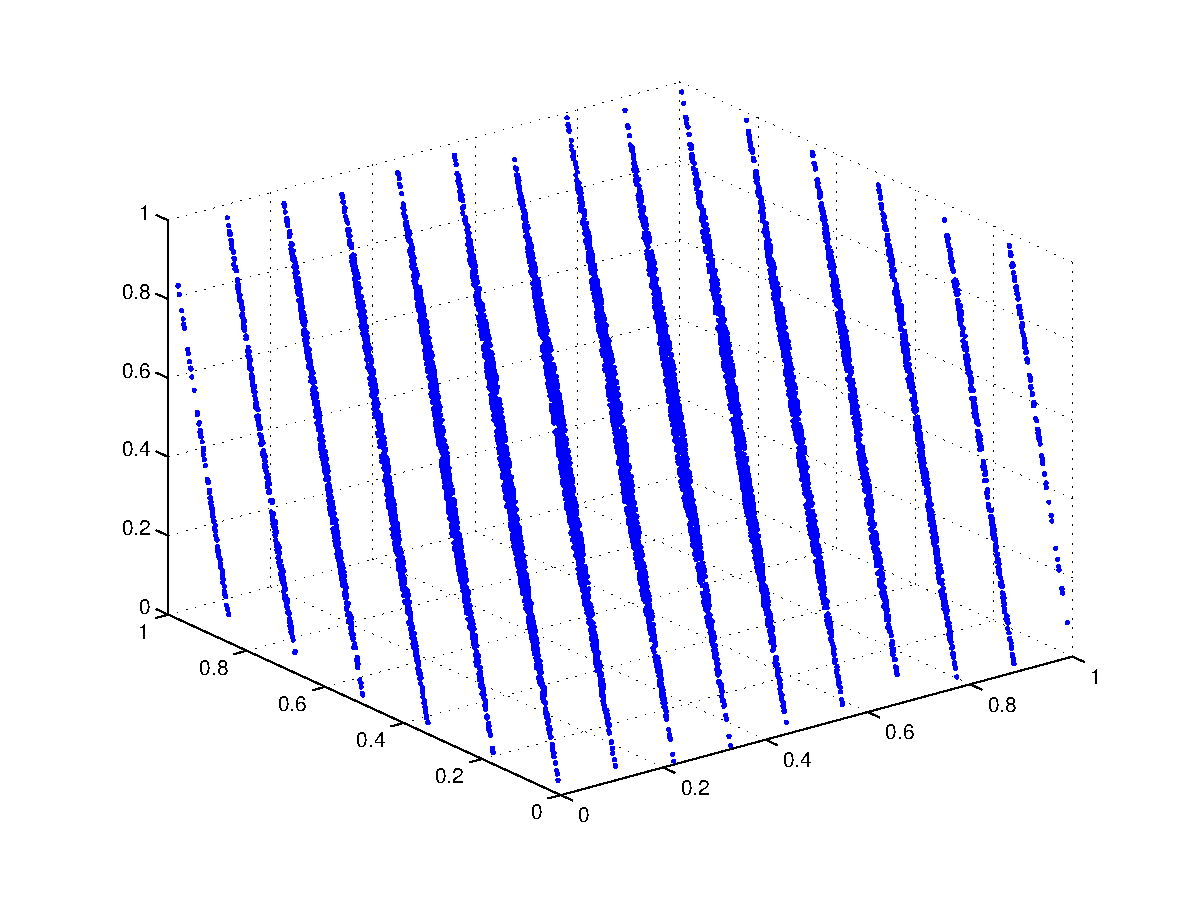
\includegraphics[width=8cm]{images/ibm_randu.eps}
	\caption{Verteilung aufeinanderfolgender Zufallszahlen des IBM Randu Algorithmus}
	\label{fig:IBMRandu}
\end{figure}

\subsubsection{Die rand() Funktion von C}
Durch die einfache und sehr effiziente Berechnung finden LCG Generatoren viel Verbreitung in der Praxis. So verwendet die C-Funktion \texttt{rand()} nach dem LCG-Algorithmus mit den Konstanten $a=1103515245$, $c=12345$, $m=2^{31}$, und dem mit der Funktion \texttt{srand()} gesetzten Startwert. \cite{rng:randFunction} Eine gängige Praxis ist es, den Startwert mit der aktuellen Systemzeit zu initialisieren. Ein entsprechendes Code-Snippet liegt im Github-Repository bei. \cite{rng:githubRepo} \\


\subsection{Lehmer Generator} \label{subsec:Lehmer}
Der Lehmer-Generator ist eine Unterart der LCG Generatoren, nach folgender Rekursionsvorschrift:

\begin{equation}
	x_{i+1} = a x_{i} \mod{m}
	\label{equ:lehmer}
\end{equation}

wobei $m$ eine Primzahl sein muss. Sie zeichnen sich gegenüber Standard LCG Generatoren durch eine höhere Periodendauer aus. David W. Hutchinson in seinem Paper \textit{``A new uniform pseudorandom number generator''} 1966 \cite{rng:Hutchinson1966} vor, das Modul  $m = 2^{31} - 1 = 2'147'483'647$ zu wählen. Damit ist der Generator in 32-bit Systemen relativ effizient umsetzbar. Eine optimale Wahl des Parameters $a$ blieb er jedoch schuldig. \\

Erst Jahre später, im Oktober 1988, publizierten Stephen K. Park und Keith W. Miller im Journal \textit{Communications of the ACM}\footnote{ACM: Association for Computing Machinery: Renommierte wissenschaftliche Gesellschaft zur Förderung der Informatik} einen Artikel \cite{rng:ParkMiller1988}, in welchem Sie genauer auf eine gute Wahl von $a$ eingingen. Sie zeigten sich in ihrem Paper \textit{`` Random number generators: good ones are hard to find.''} sehr besorgt über die gängige Praxis von Zufallsgeneratoren - insbesondere auch in Fach- und Lehrbüchern:

\begin{quote}
	\textit{Many generators have been written, most of them have demonstrably non-random characteristics, and some are embarrassingly bad.}
\end{quote}
\begin{flushright}
	- Stephen Park, Keith Miller, 1988 \cite{rng:ParkMiller1988}
\end{flushright}

Sie kritisieren insbesondere, dass, wie am Beispiel IBM gezeigt, häufig mehr Fokus auf Codeoptimierung anstatt auf die Qualität der Generatoren gelegt wird. Neben der klaren Aussage, dass das Modul $m$ unbedingt eine Primzahl sein soll, stellen Sie folgende Anforderungen an die Wahl des Faktoren $a$:

\begin{enumerate}
	\item Die Funktion $f(z) = a z \mod m$ erzeugt die maximal mögliche Periode $m$.
	\item Die komplette erzeugte Sequenz ist zufällig.
	\item $f(z)$ kann effizient auf einem 32-bit System implementiert werden.
\end{enumerate}

Aus Bedingung 3. folgt, dass die von Hutchinson \cite{rng:Hutchinson1966} vorgeschlagene Wahl von $m = 2^{31} - 1$ fast optimal für 32-bit Systeme ist. Aus den mehr als 2 Milliarden möglichen $a$ erfüllen nur einzelne alle drei Bedingungen. Bereits 1969 schlugen Lewis, Goodman, Miller \cite{rng:LewisGoodmanMiller1969} die Wahl von $a = 7^5 = 16'807$ vor, bis zum Paper von Park und Miller fand dies aber kaum Beachtung. Genau diese Kombination wurde von Park und Miller als \textbf{Minmal Standard}  für Random Number Generators bezeichnet. In der Literatur wird für diesen RNG häufig die Bezeichnung Park-Miller RNG benutzt. \\

In den 90er Jahren wurde der Park-Miller Generator von einigen Seiten kritisiert, sodass diese offiziell als neue Faktoren $a = 48271$ oder $a = 69621$ empfahlen und ausdrücklich darauf hinwiesen dass der Algorithmus nur als Minimal Standard zu verstehen ist. So hat sich dieser auch weiterhin als Standard in vielen Bibliotheken etabliert und ist eindeutig als schneller, einfacher, aber trotzdem qualitativ hochwertiger RNG zu empfehlen.

\newpage
\subsubsection{Implementation des Minimal Standard}
Eine logisch erscheinende Implementation in C sieht wie folgt aus:
\begin{lstlisting}[style=C]
	double random(int* seed) {
		const int a = 16807;
		const int m = 2147483647;
		
		*seed = (a * (*seed)) % m;
		return ((double)*seed) / m;
	}
\end{lstlisting}
wobei die Variable \texttt{seed} den aktuellen Integer Wert speichert, und die Funktion \texttt{random} einen \texttt{double}-Wert zwischen $0$ und $1$ zurückgibt. Auf den meisten Systemen wird diese Variante \textbf{nicht} funktionieren. Der maximale Wert der Multiplikation \texttt{a * (*seed)} beträgt $16807*2147483646 \approx 1.03 * 2^{45}$, was deutlich grösser als ein Integer ist. Um solche Fehler zu verhindern schlagen Park und Miller vor, jede Implementation zu prüfen indem mit $x_1 = 1$ der Wert $x_{10001} = 1043618065$ verifiziert wird. \\

Eine Möglichkeit, solche Fehler zu umgehen liegt in der Verwendung von Floating-Point Zahlen. Dabei ist anzumerken ist, dass der Modulo-Operator für Floating-Point in C nicht definiert ist, sondern die Funktion \texttt{fmod()} aus dem \texttt{math.h} Header verwendet werden muss. Trotzdem muss darauf geachtet werden, dass die Mantisse mindestens 46-bit oder grösser ist, d.h. es muss bereits der \texttt{double}-Datentyp\footnote{double: 52-bit Mantisse} anstelle von \texttt{float}\footnote{float: 23-bit Mantisse} verwendet werden. \\

Der deutlich elegantere Ansatz ist es, jegliche Werte kleiner als $2^{32}$ zu halten. Dazu wird $m$ geschrieben als

\begin{equation}
	m = aq + r
\end{equation}
mit 
\begin{equation}
	q = \lfloor m/a \rfloor \qquad \text{und} \qquad r = m \text{ mod } a
\end{equation}
Daraus ergibt sich: (Beweis, siehe \cite{rng:ParkMiller1988})
\begin{equation}
	a x \text{ mod } m = 
		\begin{cases}
			a \left(x \text{ mod } q\right) - r \lfloor x / q\rfloor & \text{wenn }\geq 0 \\
			a \left(x \text{ mod } q\right) - r \lfloor x / q\rfloor + m & \text{sonst}
		\end{cases}
\end{equation}
Damit ergeben sich Zwischenresultate bis $2^{32}$, womit eine einfache Implementation möglich ist:

\begin{lstlisting}[style=C]
	double random(int* seed) {
		const int a = 16807;
		const int m = 2147483647;
		const int q = 127773;
		const int r = 2836;
		
		int k = *seed / q;
		*seed = a * (*seed - k*q) - k*r;
		if(*seed < 0)   *seed += m;
		return (double)*seed / m;
	}
\end{lstlisting}
Diese Implementation ist nicht nur sehr schnell, sondern verfügt, wie von Park und Miller \cite{rng:ParkMiller1988} nachgewiesen, über sehr gute Eigenschaften um als Minimal Standard verwendet zu werden.

\newpage
\subsection{Mersenne-Twister} \label{subsec:MersenneTwister}
Der Mersenne-Twister Algorithmus zeichnet sich durch eine extrem hohe Periode von $2^{19937}-1 \approx 4.3 \cdot 10^{6001}$ aus. Die Periodenlänge ist eine Mersenne-Primzahl\footnote{Mersenne-Primzahl: Primzahl der Form $2^{n}-1$} und gibt dem Algorithmus den Namen. Die Ausgabesequenz ist bis zur Dimension 623 gleichverteilt, d.h. werden die ausgegebenen Zahlen als Vektoren bis Dimension 623 interpretiert, so sind diese Vektoren immer gleichverteilt. \\

Der Mersenne-Twister Algorithmus arbeitet mit 624 Zustandswörtern $Y_1 \dots Y_N$ von typischerweise 32-bit Länge. Diese Zustände werden zu Beginn des Algorithmus initialisiert. Dies wird häufig mit dem in Abschnitt \ref{subsec:RandomDev} beschriebenen Random-Device oder mit einfacheren Zufallszahlgeneratoren wie dem LCG gemacht. Je besser (d.h. zufälliger) die Initialisierung, desto früher sind die generierten Zahlen auch zufällig. Ist dies nicht gewährleistet, kann $Y[2]$ mit einem zufälligen Seed, z.B. der Uhrzeit, initialisiert werden und $800'000$ Zahlen generiert werden, bevor der Algorithmus benutzt wird. So ist eine gute Gleichverteilung sichergestellt. \\

Der Algorithmus für alle darauf folgenden Zufallszahlen $Y_i$ für $i>N$ werden wie folgt berechnet:

\begin{align}
	h &:=  Y_{i-N} - Y_{i-N} \mod{2^{31}} + Y_{i-N+1} \mod{2^{31}} \\
	Y_i &:= Y_{i-227} \oplus \left\lfloor \frac{h}{2} \right\rfloor \oplus \left( \left(h \mod{2} \right) \cdot 9908b0df_{\text{hex}}\right)
\end{align}

Um sicherzustellen, dass alle 32-bit gleichverteilt sind, werden die Zufallszahlen $Z$ aus $Y$ wie folgt berechnet: 
\begin{align}
	x &:= Y_{i} \oplus \left\lfloor \frac{Y_i}{2^{11}} \right\rfloor \\
	y &:= x \oplus \left(\left(x \cdot 2^7\right) \wedge 9d2c5680_{\text{hex}} \right) \\
	z &:= y \oplus \left(\left(y \cdot 2^{15}\right) \wedge efc60000_{\text{hex}} \right) \\
	Z_i &:= z \oplus \left\lfloor \frac{z}{2^{18}} \right\rfloor
\end{align}

Obwohl der Mersenne-Twister Algorithmus sehr kompliziert scheint, ist die Ausführung relativ schnell. Zusammen mit den bereits beschriebenen Vorteilen hat dies dazu geführt, dass der Mersenne-Twister der Standard-Zufallszahlengenerator in vielen Bibliotheken, wie z.B. der \textit{GNU Scientific Library} ist.


\subsection{Erzeugen bestimmter Verteilungen}
Wie unter \ref{subsec:numIntegration} ausgeführt, werden Integrale häufig mit der Monte Carlo Methode gelöst, indem Zufallszahlen mit einer bestimmten Verteilung generiert werden. Es werden also Methoden benötigt, beliebige Verteilungen zu erreichen. Obwohl verschiedene Möglichkeiten bestehen, ist es natürlich nicht möglich, alle Verteilungen mit vernünftigem Aufwand zu erreichen. Die einfachste Methode ist die im folgenden Abschnitt beschriebene Inversionsmethode. 

\subsubsection{Inversionsmethode}

Um aus der im Einheitsintervall $[0,1]$ gleichverteilten Zufallsvariable $z$  eine Zufallsvariable $x$ mit der Verteilungsfunktion $F_X(x)$ zu erhalten, muss F invertiert werden und auf $z$ angewandt werden.

\begin{equation}
	x = F^{-1}(z)
\end{equation}

Ist die Inversion von $F$ analytisch möglich, ist diese Methode einfach anwendbar. Es ist zwar möglich, $F$ numerisch zu invertieren, was jedoch häufig aufwändiger ist als die Anwendung anderer Methoden. \\

In Tabelle \ref{tab:verteilungen_erzeugen} sind die mit der Inversionsmethode erstellten Algorithmen zum Generieren von Zufallszahlen einiger ausgewählter Verteilungen aufgestellt.

\begin{table}[htbp]
	\centering
	\renewcommand{\arraystretch}{1.5}
	\begin{tabular}{|l|l|l|}
		\hline
		Wahrscheinlichkeitsdichte & Wertebereich & Algorithmus \\ \hline
		$f(x) = \frac{1}{b-a}$ & $[a,b[$ & $x = (b-a) \cdot z + a$ \\ \hline
		$f(x) = 2x$ & $[0,1]$ & $x = \sqrt{z}$ \\ \hline
		$f(x) = \frac{1}{k} \exp^{-x/k}$ & $]0,\infty]$ & $x = -k \ln z$ \\ \hline
		$f(x) = - \ln x$ & $[0,1[$ & $x = z_1 \cdot z_2$ \\ \hline
	\end{tabular}
	\caption{Algorithmen zur Erzeugung von Zufallszahlen $x$ aus in $[0,1]$ gleichverteilten Zufallsvariablen $z$.}
	\label{tab:verteilungen_erzeugen}
	\renewcommand{\arraystretch}{1.0}
\end{table}

\subsection{Implementation mit Boost}
Die C++ Bibliothek \textit{Boost} bietet sehr gute Möglichkeiten zum Generieren von Zufallszahlen. Es lassen sich oben vorgestellte, wie auch verschiedene weitere Generatoren auswählen. Auch die Verteilungsfunktion kann frei gewählt werden. \\

Um einen Zufallszahlengenerator zu erstellen wird als erstes eine Klasse vom gewünschten Generatortypen instanziert. Hier wird z.B. ein Mersenne-Twister mit der aktuellen Systemzeit als Seed erstellt.

\begin{lstlisting}[style=C]
static mt19937 gen(time(0));
\end{lstlisting}

Darauf wird ausgewählt, welche Verteilungsfunktion verwendet wird. Hier wird eine Gleichverteilung im Intervall $[0,1[$ erzeugt. 

\begin{lstlisting}[style=C]
static uniform_01<mt19937> dist(gen); 
\end{lstlisting}

Darauf kann die Funktion \texttt{dist()} verwendet werden um Zufallszahlen zu generieren. Der komplette Code ist im Github-Repository \cite{rng:githubRepo} abgelegt.

Detaillierte Informationen zu den Möglichkeiten mit der Boost Random-Funktion ist auf der entsprechenden Referenz-Seite zu finden \cite{rng:boostRandom}.


\newpage
\printbibliography[heading=subbibliography]
\end{refsection}


\end{document}